%\documentstyle[epsf,twocolumn]{jarticle}       %LaTeX2e仕様
\documentclass[twocolumn]{jarticle}     %pLaTeX2e仕様(platex.exeの場合)
%\documentclass[twocolumn]{ujarticle}     %pLaTeX2e仕様(uplatex.exeの場合)
%%%%%%%%%%%%%%%%%%%%%%%%%%%%%%%%%%%%%%%%%%%%%%%%%%%%%%%%%%%%%%
%%
%%  基本バージョン
%%
%%%%%%%%%%%%%%%%%%%%%%%%%%%%%%%%%%%%%%%%%%%%%%%%%%%%%%%%%%%%%%%%
\setlength{\topmargin}{-45pt}
%\setlength{\oddsidemargin}{0cm} 
\setlength{\oddsidemargin}{-7.5mm}
%\setlength{\evensidemargin}{0cm} 
\setlength{\textheight}{24.1cm}
%setlength{\textheight}{25cm} 
\setlength{\textwidth}{17.4cm}
%\setlength{\textwidth}{172mm} 
\setlength{\columnsep}{11mm}

\kanjiskip=.07zw plus.5pt minus.5pt


% 【節が変わるごとに (1.1)(1.2) … (2.1)(2.2) と数式番号をつけるとき】
%\makeatletter
%\renewcommand{\theequation}{%
%\thesection.\arabic{equation}} %\@addtoreset{equation}{section}
%\makeatother

%\renewcommand{\arraystretch}{0.95} 行間の設定

%%%%%%%%%%%%%%%%%%%%%%%%%%%%%%%%%%%%%%%%%%%%%%%%%%%%%%%%
\usepackage[dvipdfmx]{graphicx}   %pLaTeX2e仕様(\documentstyle ->\documentclass)\documentclass[dvipdfmx]{graphicx}
\usepackage[dvipdfmx]{color}
\usepackage[subrefformat=parens]{subcaption}
\usepackage{colortbl}
\usepackage{multicol}
%%%%%%%%%%%%%%%%%%%%%%%%%%%%%%%%%%%%%%%%%%%%%%%%%%%%%%%%

\begin{document}

\twocolumn[
\noindent

\hspace{1em}
\today
\hfill
\ \ 細川 岳大

\vspace{2mm}

\hrule

\begin{center}
{\Large \bf 進捗報告}
\end{center}
\hrule
\vspace{3mm}
]

% ‚ここから 文章 Start!

\section{今週やったこと}
\begin{itemize}
	\item 前回の実験の正答率についての視覚化
 	\item GAを用いたDataAugmentaion
\end{itemize}

\section{前回の実験の正答率の視覚化}
前回の実験ではDGAを用いて実験した.サブ母集団10個に対し10個体とし,全体の個体として100個体を25世代回した.
図\ref{fig:accInitVal},\ref{fig:accInitTest},\ref{fig:accLastVal},\ref{fig:accLastTest}
に正答率を示す.このとき,時間短縮のため用いた学習済みモデルの正誤も共に示した.

\begin{figure}[h]
	\centering
	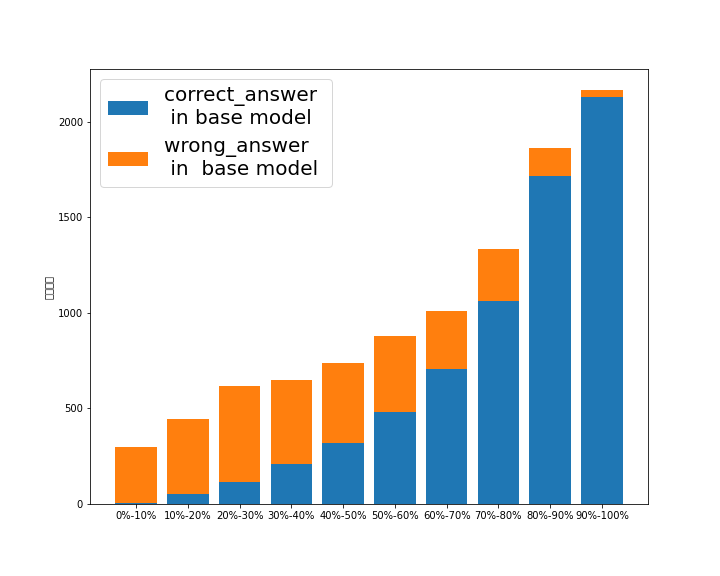
\includegraphics[scale=0.3]{graph_val_init.png}
	\caption{初期個体におけるval画像の正答率\label{fig:accInitVal}}
\end{figure}

\begin{figure}[h]
	\centering
	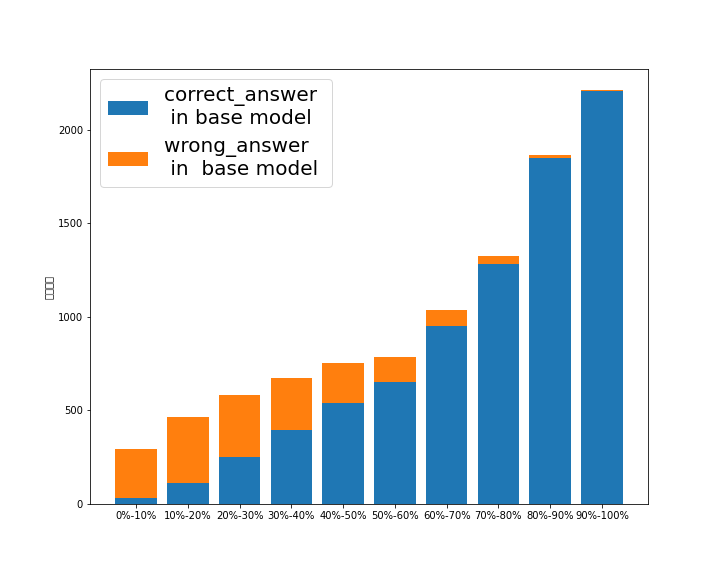
\includegraphics[scale=0.3]{graph_test_init.png}
	\caption{初期個体におけるtest画像の正答率\label{fig:accInitTest}}
\end{figure}

\begin{figure}[h]
	\centering
	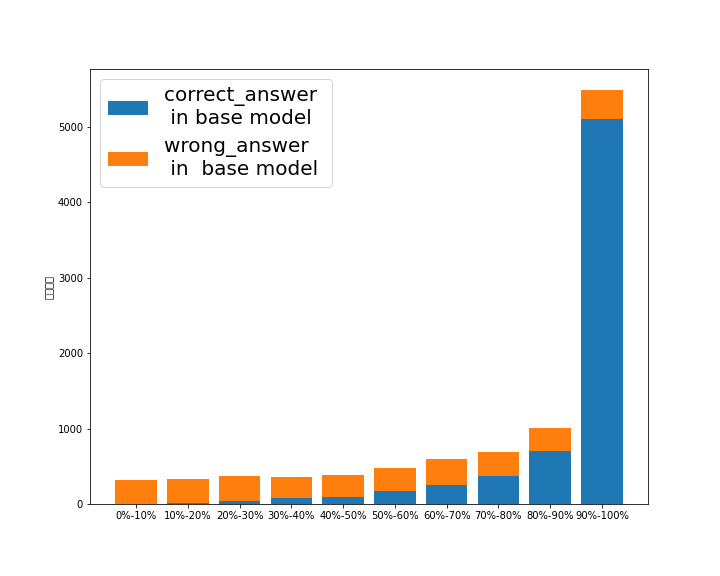
\includegraphics[scale=0.3]{graph_val_before.png}
	\caption{最終世代におけるval画像の正答率\label{fig:accLastVal}}
\end{figure}

\begin{figure}[h]
	\centering
	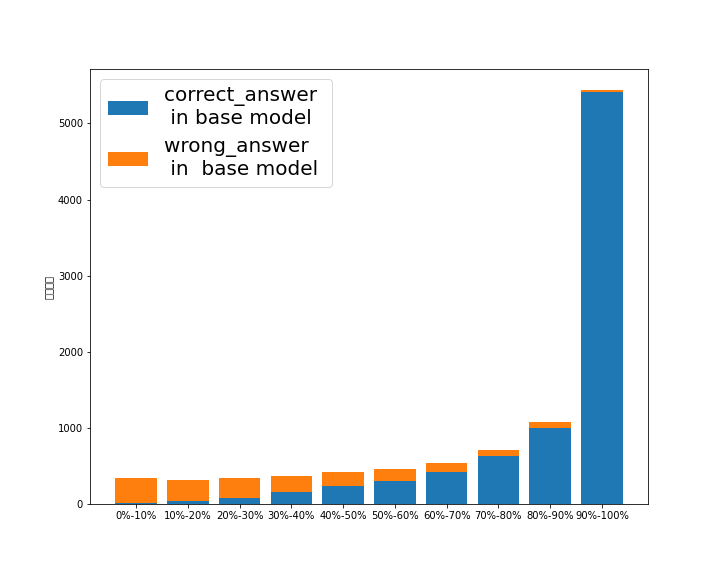
\includegraphics[scale=0.3]{graph_test_before.png}
	\caption{最終世代におけるtest画像の正答率\label{fig:accLastTest}}
\end{figure}


\section{実験}

\subsection{実験データ}
実験データはcifar10を用いて,
事前学習ではepoch数150,train\_dataを各ラベル4000枚の計40000枚使用し,GAで学習する際はepoch数30,train\_dataは各ラベル200枚のオリジナルとそれらすべてをDataAugmentaionしたものとを合わせ計4000枚とし,今回はオリジナルの2000枚は全ての個体で共通のものとした.test\_data及びvalidation\_dataは共に10000枚とした.また事前学習でのaccuracyは0.8281である.
\subsection{分散遺伝的アルゴリズム}
多様性維持として分散遺伝的アルゴリズム(Distributed Genetic Algorithm:DGA)\cite{廣安知之2002実験計画法を用いた分散遺伝的アルゴリズムのパラメータ推定}を用いる.


\subsubsection{移住}
移住間隔を3世代ごとに,移住個体数を各島2個体とした


\subsubsection{個体}
\ これまでと同様16の操作に対し強度,確率,順序をもった個体とする.

\subsubsection{選択}
\ 選択について,エリート選出によって最も適応度の高い2つの個体を選択する.なお,この二つは後述する交叉,突然変異は受けずに次の世代に追加する.
残りの選出にはトーナメントサイズが2のトーナメント選出を用いた.
 
\subsubsection{交叉}
\ 強度,確率を表す染色体については2点交叉,順序を表す染色体については部分写像交叉を用いた.2点交叉は一対の親染色体をそれぞれ同じ場所で三分割し中央の染色体を入れ替えて交叉を行う
 
\subsubsection{突然変異}
\ 強度,確率を表す染色体について,対象となる遺伝子の値を各50\%の確率に1増減させ,
 順序を表す染色体について,染色体の一部を逆順にする操作か,染色体を二つに分け前後を入れ替える操作のいずれかを行うものとした.
\subsection{適応度}
前回言われていた通り,他の島との比較を使わない,正答しにくい問題に重きを置くということを踏まえ,
事前学習における誤答した問題において個体での学習で新たに正答した数を適応度とした.

\subsection{アンサンブル学習}
\ 今回はサブ母集団ごとにもっとも適応度の高い個体を選び,それらをアンサンブルさせた.

\subsection{パラメータ}
表\ref{tb:param1}に学習パラメータを示す.
\begin{table}[h]
	\centering
	\caption{学習パラメータ\label{tb:param1}}
	\scalebox{1.0}{
		\begin{tabular}{|c||c|} \hline
			optimizer&Adam\\ \hline
			learning rate&0.001\\ \hline
			loss function&categorical\_crossentropy\\ \hline
			batch size&128\\ \hline
			epoch size&30\\ \hline
		\end{tabular}
	}
\end{table}
表\ref{tb:param_GA}にGAの設定を示す.
\begin{table}[h]
	\centering
	\caption{実験パラメータ\label{tb:param_GA}}
	\scalebox{1.0}{
		\begin{tabular}{|c|c|c|} \hline
			サブ母集団&個体数&6\\ \cline{2-3}
			&個数&6\\ \hline
			\multicolumn{2}{|c|}{総個体数}&36\\ \hline\hline
			\multicolumn{2}{|c|}{移住間隔}&3世代ごと\\ \hline
			\multicolumn{2}{|c|}{移住個体数}&2\\ \hline
			\multicolumn{2}{|c|}{世代数}&32\\ \hline
			\multicolumn{2}{|c|}{交叉率}&0.9\\ \hline\hline
			\multicolumn{3}{|c|}{突然変異率}\\ \hline
			\multicolumn{2}{|c|}{強度,確率(遺伝子ごと)}&0.06\\ \hline
			\multicolumn{2}{|c|}{順序(染色体ごと)}&0.1\\ \hline
		\end{tabular}
	}
\end{table}

\subsection{結果}
図\ref{fig:trans1},\ref{fig:trans2}に結果の推移を示す.
前回よりもGA中のアンサンブル学習の精度が3\%落ちていたが,これに関してまでtrain\_dataが40000枚からランダムに2000枚選ばれていたのに対し,今回は2000枚を固定したたのでその差が現れたのだと思われる.といっても,base\_lineと同じぐらいになってしまった理由として.base\_lineは40000枚で学習していた分アンサンブルで差が埋まったのではないかと考えられる.
一方で,得られた個体に対しtrain\_data全40000枚を用いて学習したものについて,0世代目は0.9009で,32世代目は0.911であり,これは前回の実験での最終世代が0.8947であったため,前回よりも適応度の取り方が良いのではないかと考えられる.しかし,accuracyとして1\%しか上がっていないため,まだまだ適応度の決め方に気を配る必要がある.
\\
\\

\begin{figure}[hp]
	\centering
	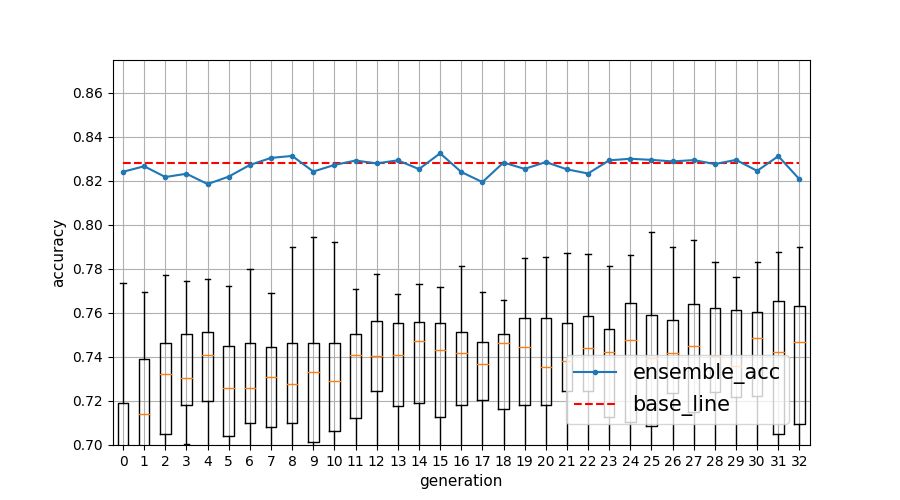
\includegraphics[scale=0.6]{graph1.png}
	\caption{valの推移\label{fig:trans1}}
\end{figure}

\begin{figure}[h]
	\centering
	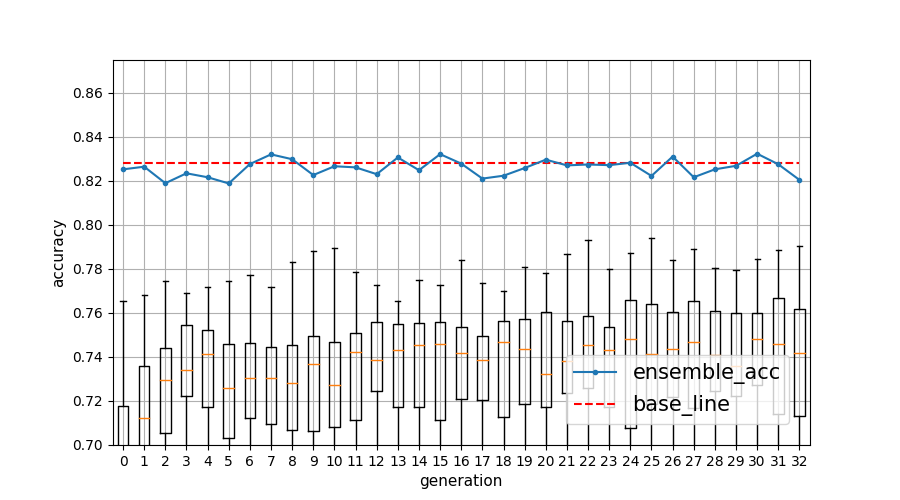
\includegraphics[scale=0.6]{graph2.png}
	\caption{testの推移\label{fig:trans2}}
\end{figure}


\section{来週の課題}
\begin{itemize}
	\item GAの適応度の取り方を工夫する
\end{itemize}

\bibliography{sa}
\bibliographystyle{unsrt}

\end{document}


